\section{一些技巧}
\subsection{如何画图}
\begin{enumerate}
  \item 二重积分 \\
  对称性+取特殊点 \\
  \item 平面 \\
    三点式画图法：\\
    画出在$x$轴,$y$轴,$z$轴的截距。\\
    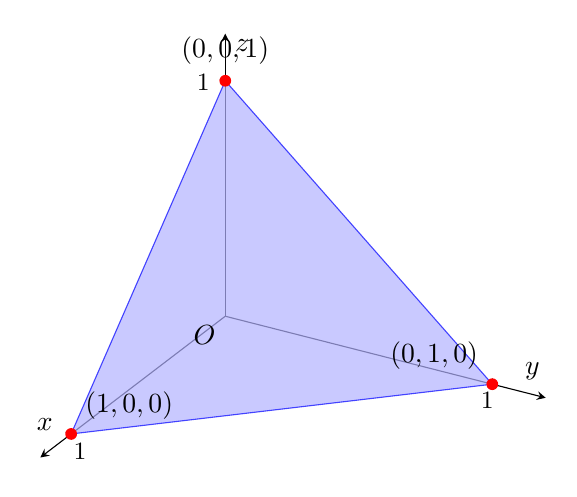
\begin{tikzpicture}
      \begin{axis}[
          axis lines=center,
          xlabel=$x$, ylabel=$y$, zlabel=$z$,
          xmin=0, xmax=1.2,
          ymin=0, ymax=1.2,
          zmin=0, zmax=1.2,
          xtick={0,1},
          ytick={0,1},
          ztick={0,1},
          ticklabel style={font=\small},
          view={120}{30},
          clip=false,
          width=8cm,
          height=8cm
        ]
        % 绘制平面 x+y+z=1 使用fill between技术
        \addplot3 [fill=blue!30, opacity=0.7, draw=blue] coordinates {
          (1,0,0) (0,1,0) (0,0,1) (1,0,0)
        };

        % 标记截距点
        \node[circle,fill=red,inner sep=1.5pt,label={above
        right:$(1,0,0)$}] at (axis cs:1,0,0) {};
        \node[circle,fill=red,inner sep=1.5pt,label={above
        left:$(0,1,0)$}] at (axis cs:0,1,0) {};
        \node[circle,fill=red,inner
        sep=1.5pt,label={above:$(0,0,1)$}] at (axis cs:0,0,1) {};

        % % 添加坐标轴标签
        % \node at (axis cs:1.3,0,0) {$x$};
        % \node at (axis cs:0,1.3,0) {$y$};
        % \node at (axis cs:0,0,1.3) {$z$};
        \node at (axis cs:0,0,0) [below left] {$O$};
      \end{axis}
    \end{tikzpicture} \\
  \item 柱面 \\
    只含两个变量,在另外一个轴上平行。\\
    % 第一个柱面: x² + y² = 1
    \boxed{\text{例1：}x^2+y^2=1}\\
    \\
    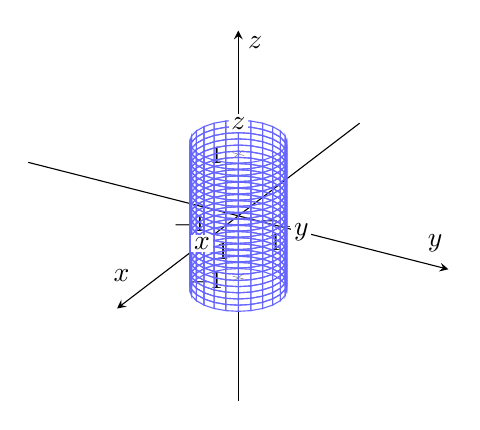
\begin{tikzpicture}
      \begin{axis}[
          axis lines=center,
          xlabel=$x$, ylabel=$y$, zlabel=$z$,
          xmin=-5, xmax=5,
          ymin=-5, ymax=5,
          zmin=-3, zmax=3,  % 减小z轴范围
          xtick={-1,0,1},
          ytick={-1,0,1},
          ztick={-1,0,1},
          view={120}{30},
          width=10cm,            % 减小画布尺寸
          height=10cm,
          ticklabel style={font=\small},
          clip=false,
        ]
        % 优化后的圆柱面绘制 - 大幅减少采样点
        \addplot3[
          mesh,
          draw=blue!60,
          fill=blue!20,
          fill opacity=0.5,
          % samples=20,        % 减少采样点
          % samples y=10,      % 减少垂直采样
          domain=0:360,      % 角度范围
          y domain=-1.2:1.2, % 高度范围
          z buffer=sort
        ] ({cos(x)}, {sin(x)}, {y});

        % 添加坐标轴标签
        \node[fill=white, inner sep=1pt] at (axis cs:1.5,0,0) {$x$};
        \node[fill=white, inner sep=1pt] at (axis cs:0,1.5,0) {$y$};
        \node[fill=white, inner sep=1pt] at (axis cs:0,0,1.5) {$z$};

        % 原点标记
        % \node at (axis cs:0,0,0) [below left] {$O$};
      \end{axis}
    \end{tikzpicture}
    \\
    \newpage
    % 第二个柱面: y² = x
    \boxed{\text{例2：}y^2=x}\\
    \\
    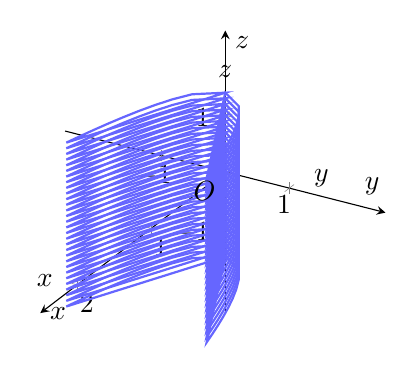
\begin{tikzpicture}
      \begin{axis}[
          axis lines=center,
          xlabel=$x$, ylabel=$y$, zlabel=$z$,
          xmin=0, xmax=2.5,
          ymin=-2.5, ymax=2.5,
          zmin=-2.5, zmax=2.5,
          xtick={0,1,2},
          ytick={-1,0,1},
          ztick={-1,0,1},
          view={120}{30},
          width=8cm,
          height=8cm,
          title style={font=\small}
        ]
        % 高效绘制抛物线柱面
        \foreach \z in {-1.5,-1.4,...,1.5} {
          \addplot3[
            thick,
            blue!60,
            samples=10,
            domain=0:1.2
          ] ({\x}, {sqrt(\x)}, {\z});
          \addplot3[
            thick,
            blue!60,
            samples=10,
            domain=0:1.2,
          ] ({\x}, {-sqrt(\x)}, {\z});
        }

        % 添加坐标轴标签
        \node at (axis cs:2.5,0,0) [right] {$x$};
        \node at (axis cs:0,1.5,0) [above] {$y$};
        \node at (axis cs:0,0,1.5) [above] {$z$};
        \node at (axis cs:0,0,0) [below left] {$O$};
      \end{axis}
    \end{tikzpicture} \\
    \\
    % 第三个柱面: z = 1 - x²
    \boxed{\text{例3：}z=1-x^2}\\
    \\
    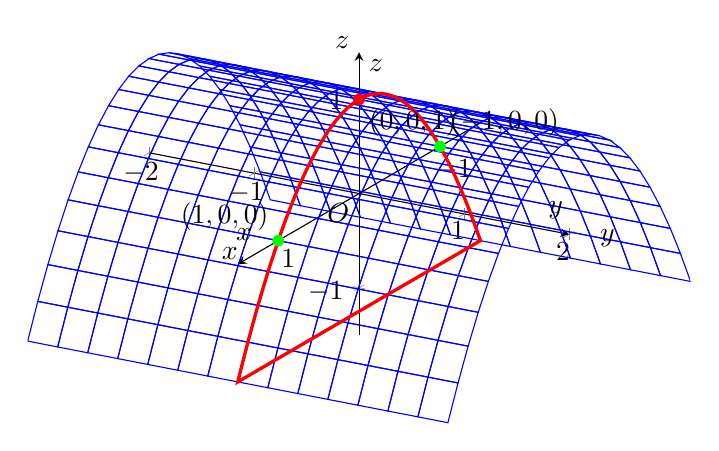
\begin{tikzpicture}
      \begin{axis}[
          axis lines=center,
          xlabel=$x$, ylabel=$y$, zlabel=$z$,
          xmin=-1.5, xmax=1.5,
          ymin=-2, ymax=2,
          zmin=-1.5, zmax=1.5,
          xtick={-1,0,1},
          ytick={-2,-1,0,1,2},
          ztick={-1,0,1},
          view={120}{30},
          width=10cm,
          height=8cm,
          title style={font=\small, yshift=2ex}
        ]
        % 高效绘制抛物柱面 - 使用线框模式
        \addplot3[
          mesh,
          samples=25,
          samples y=15,
          domain=-1.5:1.5,
          y domain=-2:2,
          % colormap={cool}{},
          draw=blue,
          line width=0.4pt
        ] {1 - x^2};

        % 添加关键曲线
        \addplot3[
          very thick,
          red,
          samples=50,
          domain=-1.5:1.5,
        ] (x, 0, {1 - x^2});

        % 添加坐标轴标签
        \node at (axis cs:1.6,0,0) [above] {$x$};
        \node at (axis cs:0,2.2,0) [right] {$y$};
        \node at (axis cs:0,0,1.6) [left] {$z$};
        \node at (axis cs:0,0,0) [below left] {$O$};

        % 标记顶点和特征点
        \node[circle,fill=red,inner sep=1.5pt] at (axis cs:0,0,1) {};
        \node[below right] at (axis cs:0,0,1) {$(0,0,1)$};

        \node[circle,fill=green,inner sep=1.5pt] at (axis cs:1,0,0) {};
        \node[above left] at (axis cs:1,0,0) {$(1,0,0)$};

        \node[circle,fill=green,inner sep=1.5pt] at (axis cs:-1,0,0) {};
        \node[above right] at (axis cs:-1,0,0) {$(-1,0,0)$};

        % % 添加方程标签
        % \node[fill=white, inner sep=2pt, rounded corners] at (axis
        % cs:0,-1.5,1.2)
        %     {$z = 1 - x^2$};
      \end{axis}
    \end{tikzpicture}
  \item 旋转曲面 \\
    含两个曲面的平方和，旋转轴为另一变量对应的轴 \\
    \boxed{\text{例1：}z=x^2+y^2} \\
    先关注$z=y^{2}$,然后绕$z$轴旋转 \\
    \\
    %画出z=y^{2}， x=0的图像
    \begin{tikzpicture}
      \begin{axis}[
          axis lines=center,
          xlabel=$x$, ylabel=$y$, zlabel=$z$,
          xmin=-0.5, xmax=0.5,
          ymin=-1.5, ymax=1.5,
          zmin=-0.5, zmax=2.5,
          xtick={0},
          ytick={-1,0,1},
          ztick={0,1,2},
          view={120}{30},
          width=8cm,
          height=8cm,
          title style={font=\small},
          title={Step 1: 先关注$z=y^{2}$}
        ]
        % 绘制抛物线曲线 (x=0, z=y^2)
        \addplot3[
          thick,
          red,
          samples=20,
          domain=-1.5:1.5,
        ] (0, x, {x^2});

        % 标记关键点
        \node[circle,fill=blue,inner sep=1.5pt,label={above
        left:$(0,0,0)$}] at (axis cs:0,0,0) {};
        \node[circle,fill=blue,inner
        sep=1.5pt,label={above:$(0,1,1)$}] at (axis cs:0,1,1) {};
        \node[circle,fill=blue,inner
        sep=1.5pt,label={below:$(0,-1,1)$}] at (axis cs:0,-1,1) {};
        \node[circle,fill=blue,inner
        sep=1.5pt,label={left:$(0,0,0)$}] at (axis cs:0,0,0) {};

        % 添加坐标轴标签
        \node at (axis cs:0.5,0,0) [right] {$x$};
        \node at (axis cs:0,1.6,0) [above] {$y$};
        \node at (axis cs:0,0,2.6) [left] {$z$};

        % 添加平面指示
        \draw[blue!30, fill=blue!10, opacity=0.5] (axis cs:0,-1.5,0)
        -- (axis cs:0,1.5,0) -- (axis cs:0,1.5,2.5) -- (axis
        cs:0,-1.5,2.5) -- cycle;
        \node[blue!80] at (axis cs:0,0.5,2) {$x=0$};

      \end{axis}
    \end{tikzpicture} \\
    之后绕$z$轴旋转，即可得到$z=x^2+y^2$的图像 \\
    %椭圆抛物面
    % \begin{tikzpicture}
    % \begin{axis}[tick label style={font=\tiny},view={120}{30},
    % axis lines =center, mark=none, axis on top, xmax=1.5, ymax=1.5,
    % zmax=0.8, width=8cm, height=8cm]
    % \addplot3 [colormap/winter, surf, z buffer=sort,
    % samples=30,domain=0:1, y domain=0:2*pi,]
    % ({x* cos(deg(y))},{x* sin(deg(y))},0.5*x^2);

    %   \node at (axis cs: 1.0,0,0) {$x$};
    %   \node at (axis cs: 0,1.0,0) {$y$};
    %   \node at (axis cs: 0,0,0.8) {$z$};
    % \end{axis}
    % \end{tikzpicture}
    \begin{tikzpicture}
      \begin{axis}[
          axis lines=center,
          xlabel=$x$, ylabel=$y$, zlabel=$z$,
          xmin=-2, xmax=2, ymin=-2, ymax=2, zmin=0, zmax=4.5,
          view={120}{30},
          % colormap={viridis}{},
          width=8cm, height=8cm,
          title={Step 2:绕$z$轴旋转得到 $z = x^2 + y^2$},
          title style={font=\small}
        ]

        % 原始抛物线
        \addplot3[very thick, red, samples=20, domain=-2:2]
        (0, x, {x^2});

        \addplot3[very thick, red, samples=20, domain=-2:2]
        (y, 0, {y^2});
        %画一条从(-1,0,4)到(1,0,4)的线段
        \draw[very thick, red] (axis cs:-2,0,4) -- (axis cs:2,0,4);

        % 添加坐标轴标签
        \node at (axis cs:2.3,0,0) [right] {$x$};
        \node at (axis cs:0,2.3,0) [above] {$y$};
        \node at (axis cs:0,0,4.8) [left] {$z$};

        % 标记关键点和轨迹
        \node[circle,fill=blue,inner sep=1.5pt] at (axis cs:0,1,1) {};
        \addplot3[thick, blue, samples=20, domain=0:360]
        ({cos(x)}, {sin(x)}, 1);

        \node[circle,fill=green,inner sep=1.5pt] at (axis cs:0,1.5,2.25) {};
        \addplot3[thick, green, samples=20, domain=0:360]
        ({1.5 * cos(x)}, {1.5 * sin(x)}, 2.25);

        \node[circle,fill=red,inner sep=1.5pt] at (axis cs:0,2,4) {};
        \addplot3[thick, red, samples=20, domain=0:360]
        ({2*cos(x)}, {2*sin(x)}, 4);

        % % 添加旋转说明
        % \draw[->, thick, green] (axis cs:0,1,1) to [bend right]
        %     node[midway, above, sloped] {rotate} (axis cs:0.7,0.7,1);
      \end{axis}
    \end{tikzpicture}

    \boxed{\text{例2：}x^2+y^2+z^2=a^2} \\
    %先关注x^2+z^2=a^2
    \begin{tikzpicture}
      \begin{axis}[
          axis lines=center,
          xlabel=$x$, ylabel=$y$, zlabel=$z$,
          xmin=-3, xmax=3, ymin=-3, ymax=3, zmin=-3,zmax=3,
          view={120}{30},
          title={Step 1:关注$x^2+y^2=a^2$,示例中$a$为$2$},
          title style={font=\small}
        ]

        \addplot3[thick, red, samples=20, domain=0:360]
        ({2*cos(x)}, 0, {2*sin(x)});

      \end{axis}
    \end{tikzpicture} \\

    %画出x^2+y^2+z^2=2^2,即一个网格球面
    \begin{tikzpicture}
        \begin{axis}[
            axis lines=center,
            xlabel=$x$, ylabel=$y$, zlabel=$z$,
            xmin=-3, xmax=3, ymin=-3, ymax=3, zmin=-3,zmax=3,
            xtick={-2,-1,0,1,2},
            ytick={-2,-1,0,1,2},
            ztick={-2,-1,0,1,2},
            view={120}{30},      % 方位角45°, 仰角30°
            % width=10cm, 
            % height=10cm,
            title={Step 2:绕$z$轴旋转得到球面},
            title style={font=\small},
        ]
            % ===== 绘制球面 =====
            \addplot3[
                surf,
                % thick,
                red,
                opacity=0.8,    % 半透明效果
                samples=30,     % 经度方向采样点
                samples y=30,   % 纬度方向采样点
                domain=0:360,   % 经度范围 (0° 到 360°)
                y domain=0:180, % 纬度范围 (0° 到 180°)
                z buffer=sort
            ] ({2*sin(y)*cos(x)}, {2*sin(y)*sin(x)}, {2*cos(y)});
            
            % ===== 标记关键点 =====
            \node[circle,fill=red,inner sep=1.5pt,label={above right:$(2,0,0)$}] at (axis cs:2,0,0) {};
            \node[circle,fill=red,inner sep=1.5pt,label={above left:$(-2,0,0)$}] at (axis cs:-2,0,0) {};
            \node[circle,fill=red,inner sep=1.5pt,label={left:$(0,2,0)$}] at (axis cs:0,2,0) {};
            \node[circle,fill=red,inner sep=1.5pt,label={right:$(0,-2,0)$}] at (axis cs:0,-2,0) {};
            \node[circle,fill=red,inner sep=1.5pt,label={above:$(0,0,2)$}] at (axis cs:0,0,2) {};
            \node[circle,fill=red,inner sep=1.5pt,label={below:$(0,0,-2)$}] at (axis cs:0,0,-2) {};
        \end{axis}
    \end{tikzpicture}

  \item 一般二次曲面 \\
    其画图方法为寻找平方和，找到平方和后化简将其当作旋转曲面对待，画出草图，再纠结具体形状 \\
    \boxed{z=\frac{x^2}{3}+\frac{y^2}{4}}\\
    如旋转曲面画法，当成$z=x^2+y^2$的旋转曲面，绕$z$轴旋转即可 \\
    最后因为是椭圆，图会扁不少\\
    \boxed{
      \frac{z^2}{2} - \frac{x^2}{3} - \frac{y^2}{4} = 0
    }
    \\
    化为\\
    \boxed{
      \frac{z^2}{2} - (\frac{1}{3}x^2 + \frac{1}{4}y^2) = 0
    }
    \\
    计算(使用例1的方法计算) \\
    \boxed{
      \frac{z^2}{2} - \frac{1}{4}y^2 = 0;
    }\\
    然后绕$z$轴旋转，即可。

  \item 其他二次曲面 \\
    \boxed{z=xy} \\
    马鞍面，可以直接记 \\
    %画出z=xy
    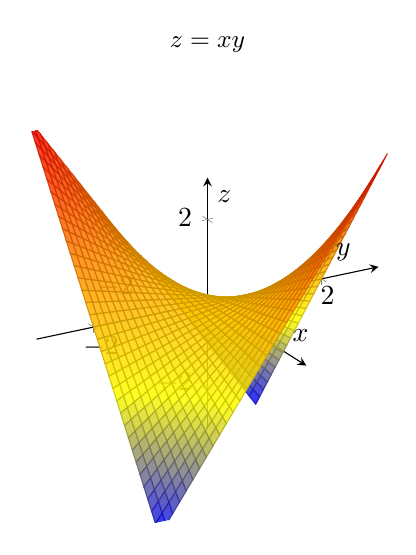
\begin{tikzpicture}
      \begin{axis}[
        axis lines=center,
        xlabel=$x$, ylabel=$y$, zlabel=$z$,
        xmin=-3, xmax=3, ymin=-3, ymax=3, zmin=-3,zmax=3,
        view={60}{30},
        title={$z=xy$},
        title style={font=\small},
        grid=major,
        grid style={dashed, gray!30}
      ]
        \addplot3[
        surf,
        opacity=0.85,   % 半透明效果
        samples=35,     % x方向采样点
        samples y=35,   % y方向采样点
        domain=-2:2,    % x范围
        y domain=-2:2,  % y范围
        % shader=interp   % 平滑着色
    ] {x*y};
      \end{axis}
    \end{tikzpicture}


\end{enumerate}

\subsection{对于某些情况的处理}
\begin{conclusion}{对于绝对值的处理}{process of abs}
\end{conclusion}


\section{综合习题}

\subsection{基础过关题}

\textbf{1.}（极限与积分综合）设 $f(x)$ 连续可导，$f(0)=0$，$f'(0)=2$。令
\[
F(x)=\int_{0}^{x} t f(x^{2}-t^{2})\,\mathrm{d}t.
\]
\begin{enumerate}[label=(\arabic*)]
\item 求 $F'(x)$；
\item 求极限 $\displaystyle\lim_{x\to 0}\frac{F(x)}{x^{4}}$。
\end{enumerate}

\boxed{\textbf{解}}
(1) 作变量代换 $u=x^{2}-t^{2}$，则 $\mathrm{d}u=-2t\,\mathrm{d}t$，$t\,\mathrm{d}t=-\frac{1}{2}\mathrm{d}u$。
当 $t=0$ 时 $u=x^{2}$；$t=x$ 时 $u=0$。于是
\[
F(x)=\int_{x^{2}}^{0} f(u)\cdot\Bigl(-\frac{1}{2}\Bigr)\mathrm{d}u
     =\frac{1}{2}\int_{0}^{x^{2}} f(u)\,\mathrm{d}u.
\]
由变上限积分求导公式，
\[
F'(x)=\frac{1}{2}f(x^{2})\cdot 2x = xf(x^{2}).
\]

(2) 由 $f(0)=0$，$f'(0)=2$ 知 $f(u)=2u+o(u)$（$u\to 0$）。故
\[
\int_{0}^{x^{2}} f(u)\,\mathrm{d}u
=\int_{0}^{x^{2}} \bigl[2u+o(u)\bigr]\mathrm{d}u
=x^{4}+o(x^{4}),
\]
从而 $F(x)=\frac{1}{2}x^{4}+o(x^{4})$。因此
\[
\lim_{x\to 0}\frac{F(x)}{x^{4}}=\frac{1}{2}.
\]


\textbf{2.}（导数与积分综合）设 $f(x)$ 可导，且满足积分方程
\[
\int_{0}^{x} (x-t)f'(t)\,\mathrm{d}t = f(x)-\sin x,
\]
以及 $f(0)=0$。求 $f(x)$ 的表达式。

\boxed{\textbf{解}}
记 $I(x)=\displaystyle\int_{0}^{x}(x-t)f'(t)\,\mathrm{d}t$，则原方程为 $I(x)=f(x)-\sin x$。

求导得
\[
I'(x)=\frac{\mathrm{d}}{\mathrm{d}x}\Bigl[x\int_{0}^{x}f'(t)\,\mathrm{d}t-\int_{0}^{x}tf'(t)\,\mathrm{d}t\Bigr]
     =\int_{0}^{x}f'(t)\,\mathrm{d}t + xf'(x) - xf'(x)
     =f(x)-f(0)=f(x).
\]
另一方面，对原方程两边求导：$I'(x)=f'(x)-\cos x$。于是
\[
f(x)=f'(x)-\cos x\quad\Longrightarrow\quad f'(x)-f(x)=\cos x.
\]

这是一阶线性微分方程，积分因子为 $e^{-x}$：
\[
\bigl(e^{-x}f(x)\bigr)' = e^{-x}\cos x.
\]
积分得
\[
e^{-x}f(x)=\int_{0}^{x} e^{-t}\cos t\,\mathrm{d}t
          =\frac{e^{-x}}{2}(\sin x-\cos x)+\frac{1}{2}.
\]
故
\[
f(x)=\frac{1}{2}(\sin x-\cos x)+\frac{1}{2}e^{x}.
\]


\textbf{3.}（极限与定积分综合）求极限
\[
\lim_{n\to\infty}\frac{1}{n^{2}}\sum_{k=1}^{n}\sqrt{n^{2}-k^{2}}.
\]

\boxed{\textbf{解}}
将和式改写为 Riemann 和的形式：
\[
\frac{1}{n^{2}}\sum_{k=1}^{n}\sqrt{n^{2}-k^{2}}
=\frac{1}{n}\sum_{k=1}^{n}\sqrt{1-\Bigl(\frac{k}{n}\Bigr)^{2}}.
\]
取分割 $0<\frac{1}{n}<\frac{2}{n}<\cdots<\frac{n}{n}=1$，被积函数 $f(x)=\sqrt{1-x^{2}}$，则
\[
\lim_{n\to\infty}\frac{1}{n}\sum_{k=1}^{n}\sqrt{1-\Bigl(\frac{k}{n}\Bigr)^{2}}
=\int_{0}^{1}\sqrt{1-x^{2}}\,\mathrm{d}x.
\]
该定积分为单位圆的四分之一面积，故
\[
\int_{0}^{1}\sqrt{1-x^{2}}\,\mathrm{d}x = \frac{\pi}{4}.
\]


\subsection{综合提高题}

\textbf{4.}（微分方程与级数综合）用幂级数方法求解初值问题
\[
y''+xy'+y=0,\qquad y(0)=1,\; y'(0)=0.
\]
将解写成幂级数形式，写出前5项，并指出该级数的收敛半径。

\boxed{\textbf{解}}
设 $y=\displaystyle\sum_{n=0}^{\infty} a_{n}x^{n}$，则
\[
y'=\sum_{n=1}^{\infty} na_{n}x^{n-1},\qquad
y''=\sum_{n=2}^{\infty} n(n-1)a_{n}x^{n-2}.
\]
代入方程：
\[
\sum_{n=2}^{\infty} n(n-1)a_{n}x^{n-2}
+x\sum_{n=1}^{\infty} na_{n}x^{n-1}
+\sum_{n=0}^{\infty} a_{n}x^{n}=0.
\]
将第一项指标平移：令 $m=n-2$，得 $\sum_{m=0}^{\infty}(m+2)(m+1)a_{m+2}x^{m}$。
各项统一为 $x^{n}$ 的幂：
\[
\sum_{n=0}^{\infty}\bigl[(n+2)(n+1)a_{n+2}+na_{n}+a_{n}\bigr]x^{n}=0,
\]
其中 $na_{n}$ 项仅从 $n=1$ 开始，但当 $n=0$ 时该项自然为零。比较系数得递推公式
\[
(n+2)(n+1)a_{n+2}+(n+1)a_{n}=0
\;\Longrightarrow\;
a_{n+2}=-\frac{a_{n}}{n+2}\quad (n=0,1,2,\ldots).
\]

初始条件：$a_{0}=y(0)=1$，$a_{1}=y'(0)=0$。由 $a_{1}=0$ 知所有奇次项均为零。逐次计算偶次项：
\[
a_{2}=-\frac{a_{0}}{2}=-\frac{1}{2},\quad
a_{4}=-\frac{a_{2}}{4}=\frac{1}{8},\quad
a_{6}=-\frac{a_{4}}{6}=-\frac{1}{48},\quad
a_{8}=-\frac{a_{6}}{8}=\frac{1}{384}.
\]
故
\[
y(x)=1-\frac{x^{2}}{2}+\frac{x^{4}}{8}-\frac{x^{6}}{48}+\frac{x^{8}}{384}-\cdots
     =e^{-x^{2}/2}.
\]
（事实上，直接验证可知 $y=e^{-x^{2}/2}$ 满足原方程。）该级数为指数函数的幂级数，收敛半径 $R=+\infty$。


\textbf{5.}（多元函数与曲线积分综合）验证曲线积分
\[
I=\int_{L} (3x^{2}y+e^{y})\,\mathrm{d}x+(x^{3}+xe^{y}-2y)\,\mathrm{d}y
\]
在全平面上与路径无关，并求从原点 $O(0,0)$ 到点 $A(1,1)$ 的积分值。

\boxed{\textbf{解}}
记 $P=3x^{2}y+e^{y}$，$Q=x^{3}+xe^{y}-2y$。则
\[
\frac{\partial P}{\partial y}=3x^{2}+e^{y},\qquad
\frac{\partial Q}{\partial x}=3x^{2}+e^{y}.
\]
由于 $\frac{\partial P}{\partial y}=\frac{\partial Q}{\partial x}$ 在全平面恒成立，积分与路径无关。

求势函数 $u(x,y)$ 使 $\mathrm{d}u=P\mathrm{d}x+Q\mathrm{d}y$。由 $\frac{\partial u}{\partial x}=P$ 得
\[
u(x,y)=\int (3x^{2}y+e^{y})\,\mathrm{d}x = x^{3}y+xe^{y}+\varphi(y).
\]
代入 $\frac{\partial u}{\partial y}=Q$：
\[
x^{3}+xe^{y}+\varphi'(y)=x^{3}+xe^{y}-2y\;\Longrightarrow\; \varphi'(y)=-2y,
\]
故 $\varphi(y)=-y^{2}+C$。取 $C=0$ 得 $u(x,y)=x^{3}y+xe^{y}-y^{2}$。于是
\[
I=u(1,1)-u(0,0)=(1+e-1)-0=e.
\]


\textbf{6.}（积分与级数综合）将函数
\[
f(x)=\int_{0}^{x} \frac{\ln(1+t)}{t}\,\mathrm{d}t
\]
展开为 $x$ 的幂级数，并求常数项级数 $\displaystyle\sum_{n=1}^{\infty}\frac{(-1)^{n-1}}{n^{2}}$ 的和。

\boxed{\textbf{解}}
由对数函数的幂级数展开式 $\ln(1+t)=\displaystyle\sum_{n=1}^{\infty}\frac{(-1)^{n-1}}{n}t^{n}$（$|t|<1$），有
\[
\frac{\ln(1+t)}{t}=\sum_{n=1}^{\infty}\frac{(-1)^{n-1}}{n}t^{n-1},\quad |t|<1.
\]
逐项积分（幂级数在其收敛区间内可逐项积分）：
\[
f(x)=\sum_{n=1}^{\infty}\frac{(-1)^{n-1}}{n}\cdot\frac{x^{n}}{n}
     =\sum_{n=1}^{\infty}\frac{(-1)^{n-1}}{n^{2}}x^{n},\quad |x|\leq 1.
\]
（当 $x=1$ 时级数为交错级数，由 Leibniz 判别法知其收敛；$x=-1$ 时类似。）

令 $x=1$，则
\[
f(1)=\sum_{n=1}^{\infty}\frac{(-1)^{n-1}}{n^{2}}.
\]
另一方面，
\[
\sum_{n=1}^{\infty}\frac{(-1)^{n-1}}{n^{2}}
=\sum_{n=1}^{\infty}\frac{1}{n^{2}}-2\sum_{n=1}^{\infty}\frac{1}{(2n)^{2}}
=\frac{\pi^{2}}{6}-\frac{2}{4}\cdot\frac{\pi^{2}}{6}
=\frac{\pi^{2}}{12}.
\]
（也可由 $f(1)=\int_{0}^{1}\frac{\ln(1+t)}{t}\mathrm{d}t$ 及二重积分或 dilog 函数得知其值为 $\frac{\pi^{2}}{12}$。）


\textbf{7.}（多元极值与重积分综合）设 $a,b,c>0$。在椭球面
\[
\frac{x^{2}}{a^{2}}+\frac{y^{2}}{b^{2}}+\frac{z^{2}}{c^{2}}=1
\]
的第一卦限部分上求一点 $P(x_{0},y_{0},z_{0})$，使得过该点的切平面与三个坐标平面所围成的四面体体积最小，并求该最小体积。

\boxed{\textbf{解}}
椭球面在点 $P(x_{0},y_{0},z_{0})$ 处的切平面方程为
\[
\frac{x_{0}x}{a^{2}}+\frac{y_{0}y}{b^{2}}+\frac{z_{0}z}{c^{2}}=1.
\]
切平面在三个坐标轴上的截距分别为
\[
X=\frac{a^{2}}{x_{0}},\quad Y=\frac{b^{2}}{y_{0}},\quad Z=\frac{c^{2}}{z_{0}}.
\]
四面体体积为
\[
V=\frac{1}{6}XYZ=\frac{a^{2}b^{2}c^{2}}{6x_{0}y_{0}z_{0}}.
\]
要使 $V$ 最小，需使乘积 $x_{0}y_{0}z_{0}$ 最大。点 $P$ 在椭球面上，满足约束
\[
\frac{x_{0}^{2}}{a^{2}}+\frac{y_{0}^{2}}{b^{2}}+\frac{z_{0}^{2}}{c^{2}}=1,\quad x_{0},y_{0},z_{0}>0.
\]

由 AM--GM 不等式：
\[
1=\frac{x_{0}^{2}}{a^{2}}+\frac{y_{0}^{2}}{b^{2}}+\frac{z_{0}^{2}}{c^{2}}
  \geq 3\sqrt[3]{\frac{x_{0}^{2}y_{0}^{2}z_{0}^{2}}{a^{2}b^{2}c^{2}}},
\]
等号成立当且仅当 $\frac{x_{0}}{a}=\frac{y_{0}}{b}=\frac{z_{0}}{c}$。代入椭球面方程得
\[
3\Bigl(\frac{x_{0}}{a}\Bigr)^{2}=1\;\Longrightarrow\;
\frac{x_{0}}{a}=\frac{y_{0}}{b}=\frac{z_{0}}{c}=\frac{1}{\sqrt{3}}.
\]
故所求点为 $P\!\left(\frac{a}{\sqrt{3}},\frac{b}{\sqrt{3}},\frac{c}{\sqrt{3}}\right)$，此时
\[
x_{0}y_{0}z_{0}=\frac{abc}{3\sqrt{3}},
\]
最小体积为
\[
V_{\min}= \frac{a^{2}b^{2}c^{2}}{6}\cdot\frac{3\sqrt{3}}{abc}
        =\frac{\sqrt{3}}{2}\,abc.
\]


\subsection{真题风格与综合训练}

\textbf{8.}（\boxed{\textbf{真题风格}}，极限与积分与级数综合）设 $F(x)=\displaystyle\int_{0}^{x} e^{-t^{2}}\,\mathrm{d}t$。
\begin{enumerate}[label=(\arabic*)]
\item 将 $F(x)$ 展开为 $x$ 的幂级数，并求其收敛域；
\item 求极限 $\displaystyle\lim_{x\to 0}\frac{F(x)-x+\frac{x^{3}}{3}}{x^{5}}$。
\end{enumerate}

\boxed{\textbf{解}}
(1) 由指数函数的幂级数展开 $e^{u}=\displaystyle\sum_{n=0}^{\infty}\frac{u^{n}}{n!}$（$|u|<\infty$），令 $u=-t^{2}$ 得
\[
e^{-t^{2}}=\sum_{n=0}^{\infty}\frac{(-1)^{n}}{n!}t^{2n},
\]
收敛半径为 $+\infty$。逐项积分：
\[
F(x)=\int_{0}^{x}\sum_{n=0}^{\infty}\frac{(-1)^{n}}{n!}t^{2n}\,\mathrm{d}t
     =\sum_{n=0}^{\infty}\frac{(-1)^{n}}{n!}\cdot\frac{x^{2n+1}}{2n+1}
     =x-\frac{x^{3}}{3}+\frac{x^{5}}{10}-\frac{x^{7}}{42}+\cdots.
\]
由于幂级数逐项积分后收敛半径不变，收敛域为 $(-\infty,+\infty)$（即 $R=+\infty$）。

(2) 由 (1) 中的展开式，
\[
F(x)-x+\frac{x^{3}}{3}
=\frac{x^{5}}{10}-\frac{x^{7}}{42}+\cdots
=\frac{x^{5}}{10}+o(x^{5})\quad (x\to 0).
\]
因此
\[
\lim_{x\to 0}\frac{F(x)-x+\frac{x^{3}}{3}}{x^{5}}
=\lim_{x\to 0}\frac{\frac{x^{5}}{10}+o(x^{5})}{x^{5}}
=\frac{1}{10}.
\]


\textbf{9.}（\boxed{\textbf{真题风格}}，曲线积分与微分方程综合）设 $f(x)$ 具有二阶连续导数，且对平面上任意一条分段光滑的简单闭曲线 $L$，均有
\[
\oint_{L} \bigl[e^{x}f'(x)+y^{2}\bigr]\,\mathrm{d}y
          +\bigl[-y\,e^{x}f(x)\bigr]\,\mathrm{d}x = 0.
\]
已知 $f(0)=0$，$f'(0)=1$，求 $f(x)$ 的表达式。

\boxed{\textbf{解}}
记 $P=-y\,e^{x}f(x)$，$Q=e^{x}f'(x)+y^{2}$。由题设，对任意闭曲线 $L$ 积分恒为零，根据 Green 公式的逆定理（或曲线积分与路径无关的充要条件），在全平面上应有
\[
\frac{\partial Q}{\partial x}=\frac{\partial P}{\partial y}.
\]
计算偏导数：
\[
\frac{\partial Q}{\partial x}=e^{x}f'(x)+e^{x}f''(x),\qquad
\frac{\partial P}{\partial y}=-e^{x}f(x).
\]
令两者相等：
\[
e^{x}\bigl[f''(x)+f'(x)\bigr]=-e^{x}f(x)
\;\Longrightarrow\;
f''(x)+f'(x)+f(x)=0.
\]

这是二阶常系数齐次线性微分方程，特征方程为 $r^{2}+r+1=0$，解得
\[
r=\frac{-1\pm i\sqrt{3}}{2}.
\]
故通解为
\[
f(x)=e^{-x/2}\Bigl(C_{1}\cos\frac{\sqrt{3}}{2}x+C_{2}\sin\frac{\sqrt{3}}{2}x\Bigr).
\]

由初始条件：$f(0)=C_{1}=0$；求导得
\[
f'(x)=-\frac{1}{2}e^{-x/2}\Bigl(C_{2}\sin\frac{\sqrt{3}}{2}x\Bigr)
      +e^{-x/2}\cdot\frac{\sqrt{3}}{2}C_{2}\cos\frac{\sqrt{3}}{2}x,
\]
故 $f'(0)=\frac{\sqrt{3}}{2}C_{2}=1$，$C_{2}=\frac{2}{\sqrt{3}}$。因此
\[
f(x)=\frac{2}{\sqrt{3}}e^{-x/2}\sin\frac{\sqrt{3}}{2}x.
\]


\textbf{10.}（\boxed{\textbf{真题风格}}，极限与积分与级数综合）设 $a_{n}=\displaystyle\int_{0}^{1} x^{n}(1-x)^{n}\,\mathrm{d}x$，$n=0,1,2,\ldots$。
\begin{enumerate}[label=(\arabic*)]
\item 求 $a_{n}$ 的表达式（用 $n$ 表示）；
\item 求极限 $\displaystyle\lim_{n\to\infty}\sqrt{n}\cdot 4^{n}a_{n}$；
\item 求幂级数 $\displaystyle\sum_{n=0}^{\infty} a_{n}x^{n}$ 的收敛半径。
\end{enumerate}

\boxed{\textbf{解}}
(1) 作变量代换 $t=1-x$ 或直接利用 Beta 函数：
\[
a_{n}=\int_{0}^{1} x^{n}(1-x)^{n}\,\mathrm{d}x
     =B(n+1,n+1)
     =\frac{\Gamma(n+1)\,\Gamma(n+1)}{\Gamma(2n+2)}
     =\frac{(n!)^{2}}{(2n+1)!}.
\]

(2) 利用 Stirling 公式 $n!\sim\sqrt{2\pi n}\bigl(\frac{n}{e}\bigr)^{n}$（$n\to\infty$）：
\[
\begin{aligned}
a_{n}&\sim\frac{2\pi n\left(\frac{n}{e}\right)^{2n}}
               {\sqrt{2\pi(2n+1)}\left(\frac{2n+1}{e}\right)^{2n+1}}
      \sim\frac{\sqrt{\pi n}\left(\frac{n}{e}\right)^{2n}}
               {2^{2n}\sqrt{n}\left(\frac{n}{e}\right)^{2n}\cdot\frac{2}{e}}
      =\frac{\sqrt{\pi}}{2^{2n+1}\sqrt{n}}.
\end{aligned}
\]
（详细：$(2n+1)!\sim(2n)(2n)!\sim 2n\cdot\sqrt{4\pi n}\bigl(\frac{2n}{e}\bigr)^{2n}
      =2^{2n+1}\sqrt{\pi}\,n^{2n+\frac{1}{2}}e^{-2n}$，与分子 $(n!)^{2}\sim 2\pi n^{2n+1}e^{-2n}$ 相除即得。）

因此
\[
4^{n}a_{n}=2^{2n}a_{n}\sim\frac{\sqrt{\pi}}{2\sqrt{n}},
\qquad
\sqrt{n}\cdot 4^{n}a_{n}\to\frac{\sqrt{\pi}}{2}\quad (n\to\infty).
\]

(3) 幂级数的收敛半径 $R$ 满足
\[
\frac{1}{R}=\lim_{n\to\infty}\left|\frac{a_{n+1}}{a_{n}}\right|.
\]
计算：
\[
\frac{a_{n+1}}{a_{n}}
=\frac{[(n+1)!]^{2}}{(2n+3)!}\cdot\frac{(2n+1)!}{(n!)^{2}}
=\frac{(n+1)^{2}}{(2n+3)(2n+2)}
\longrightarrow \frac{1}{4}\quad (n\to\infty).
\]
故 $R=4$，即幂级数的收敛半径为 $4$。
